\chapter{Metodologia}
\label{chap:metodologia}

Neste Capítulo, é apresentada a classificação de pesquisa na seção \ref{sec:classificacaoDaPesquisa}, classificando-a de acordo com a sua abordagem, sua natureza, seus objetivos e procedimentos. A seção \ref{sec:metodologiaDeDesenvolvimentoDeSoftware} apresenta a metodologia de desenvolvimento de software aplicada aos cenários. A seção \ref{sec:procedimentosMetodológicos} apresenta os procedimentos metodológicos utilizados na construção do trabalho.


\begin{comment}
	A seção \ref{sec:metodologiaDeDesenvolvimentoDeSoftware} apresenta a metodologia de desenvolvimento de software que será utilizada para o TCC2. A seção \ref{sec:procedimentosMetodológicos} apresenta os procedimentos metodológicos para o desenvolvimento desse trabalho, procurando detalhar o fluxo de atividades bem como o cronograma de ambos, TCC1 e TCC2.
\end{comment}
  

\section{Classificação da Pesquisa}
\label{sec:classificacaoDaPesquisa}

A pesquisa científica pode ser classificada de acordo com sua abordagem, sua natureza, seus objetivos e seus procedimentos técnicos \cite{gerhardt2009metodos}. Portanto, nessa seção, procura-se enquadrar a classificação de pesquisa do presente trabalho, definindo-a quanto à Abordagem (seção \ref{sub:abordagemDePesquisa}); à Natureza de (seção \ref{sub:naturezaDePesquisa}), aos Objetivos (seção \ref{sub:objetivosDePesquisa}) e aos Procedimentos técnicos (seção \ref{sub:procedimentosDePesquisa}).

\subsection{Abordagem de Pesquisa}
\label{sub:abordagemDePesquisa}

Segundo \cite{gerhardt2009metodos}, a pesquisa qualitativa preocupa-se com os aspectos da realidade que não podem ser quantificados, centrando-se na compreensão e explicação da dinâmica das relações sociais. Nela, há três características fundamentais para prosseguir com os estudos \cite{mazzotti1991planejamento}:

\begin{itemize}
	\item \textit{Visão holística:} a compreensão de um comportamento ou evento só é possível com o entendimento das inter-relações que surgem dentro do contexto da pesquisa;
	\item \textit{Abordagem indutiva:} o pesquisador parte de observações mais livres, deixando que as dimensões e categorias de interesse surjam progressivamente durante todo o processo de coleta e análise dos dados;
	\item \textit{Investigação naturalística:} a intervenção do pesquisador, no contexto observado, é reduzida ao mínimo.
\end{itemize}

A abordagem de pesquisa quantitativa possui perspectiva no pensamento lógico positivista, tentando enfatizar o raciocínio dedutivo, as regras da lógica e os atributos mensuráveis registrados por um indivíduo \cite{gerhardt2009metodos}. 

A abordagem de pesquisa qualitativa foi utilizada na execução deste trabalho junto com aspectos da pesquisa quantitativa, formando então, uma abordagem híbrida. Considerando que, para a execução da pesquisa, o autor tem a necessidade de realizar a descrição dos principais subtipos de RNFs de Segurança, visando a estruturação de um Catálogo de Segurança utilizando o NFR \textit{Framework}, bem como, compreender e explicar os impactos entre os RNFs no Padrão Arquitetural MVC.  

\subsection{Natureza de Pesquisa}
\label{sub:naturezaDePesquisa}

Essa pesquisa foi caracterizada como uma \textbf{pesquisa aplicada}, pois os conhecimentos gerados são voltados para a aplicação prática \cite{gerhardt2009metodos}, visando auxiliar os especialistas na especificação dos RNFs de segurança, quando uma arquitetura é imposta. 

\subsection{Objetivos de Pesquisa}
\label{sub:objetivosDePesquisa}

Quanto aos objetivos, essa pesquisa pode ser classificada como \textbf{pesquisa explicativa}, pois, segundo \cite{gil2002elaborar}, “... este tipo de pesquisa preocupa-se em identificar os fatores que determinam ou que contribuem para a ocorrência dos fenômenos...”, ou seja, explicou-se como o Padrão Arquitetural MVC pode ser impactado pelos RNFs, demonstrado pelo Catálogo de Segurança.

\subsection{Procedimentos Técnicos de Pesquisa}
\label{sub:procedimentosDePesquisa}

A \textbf{pesquisa bibliográfica} foi um dos procedimentos técnicos de pesquisa utilizados, como é evidente no Capítulo \ref{chap:referencialTeorico}, onde foi apresentado todo o levantamento teórico que serviu de insumo para a execução desse trabalho. 

Fonseca descreve o procedimento técnico de pesquisa como:

\begin{citacao}
	“\textit{... esse tipo de procedimento trata-se do levantamento de referências teóricas já analisadas, e publicadas por meio de escritos e eletrônicos, como livros, artigos científicos, páginas de web sites. Qualquer trabalho científico inicia-se com uma pesquisa bibliográfica, que permite ao pesquisador conhecer o que já estudou sobre o assunto}”.
	\cite[p.35]{fonseca2002metodologia}
\end{citacao}
 
 
Outro procedimento técnico de pesquisa adotado foi a \textbf{pesquisa-ação}, pois trata-se da participação planejada do autor em uma situação problemática a ser investigada \cite{fonseca2002metodologia}. O autor participou ativamente do levantamento dos conceitos teóricos, adquirindo consigo uma série de conhecimentos que serviu como base para construção do Catálogo de Segurança e que, foi validado, através da criação e aplicação em cenários. 
 

\section{Metodologia de desenvolvimento de software aplicada aos cenários}
\label{sec:metodologiaDeDesenvolvimentoDeSoftware}


A metodologia de desenvolvimento de software utilizada foi o  \textbf{\textit{scrum} com adaptações}, trata-se de uma metodologia de desenvolvimento ágil utilizada para a gestão e planejamento de projetos de software \cite{schwaber2002agile}. 

O \textit{scrum} trata os projetos de forma iterativa e incremental, entregando ao final de cada \textit{sprint}\footnote[1]{Curto período de tempo em que são realizadas as atividades de desenvolvimento de software, é indicado que seja de 2 a 4 semanas \cite{schwaber2002agile}.} uma versão funcional do software com o incremento de uma nova funcionalidade \cite{schwaber2002agile}. Para a execução do desenvolvimento do software nos cenários, cada cenário possuiu a duração de 3 semanas e foi tratado como uma \textit{sprint}, iniciando no mês de Agosto e encerrando em Novembro.  
 
Outro conceito do \textit{scrum} utilizado foi o \textit{product backlog}\footnote[2]{Lista de funcionalidades a serem implementadas no projeto de software, não necessita estar preenchida por completo no inicio do projeto, pois essa lista cresce a medida que se aprende mais sobre o produto de software \cite{schwaber2002agile}.}. Para execução deste trabalho foi aplicado o conceito de \textit{product backlog} para os cenários.

Com base no \textit{product backlog} o \textit{scrum team}\footnote[3]{Um time scrum é definido por uma equipe de pessoas variando de 6 a 10 pessoas \cite{schwaber2002agile}. No presente trabalho o \textit{scrum team} sofre adaptação para somente uma única pessoa “o autor”, mas o termo será utilizado para referir-se diretamente ao autor.} realizou o planejamento da \textit{sprint}, de acordo com as funcionalidades mais relevantes, tendo como base o contexto definido em cada cenário. 

As reuniões de retrospectiva e revisão de \textit{sprint} ocorreram duas vezes dentro da \textit{sprint}, foram reuniões semanais de ponto de controle com os orientadores as quais apresentava-se o que foi feito, o que não foi feito, e o porquê não foi feito, no decorrer da \textit{sprint}. 

O Kanban é um método ágil que promove ao \textit{scrum team} e aos \textit{stakeholders} a visão geral da gestão do estado de implementação das funcionalidades \cite{prikladnicki2014metodos}. Foi utilizado para controle visual do fluxo das atividades do desenvolvimento das funcionalidades para os cenários, dividindo suas colunas da seguinte maneira: “A fazer”, “Fazendo” e “Feito”.

\pagebreak

\section{Procedimentos Metodológicos}
\label{sec:procedimentosMetodológicos}

Para o desenvolvimento deste trabalho foi realizado um conjunto de atividades para que o Catálogo de Segurança pudesse ser elaborado e aplicado em cenários. Portanto, essas atividades foram modeladas em notação BPMN, com intuito de detalhar o fluxo de execução.

\begin{figure}[h!]
	\centering
	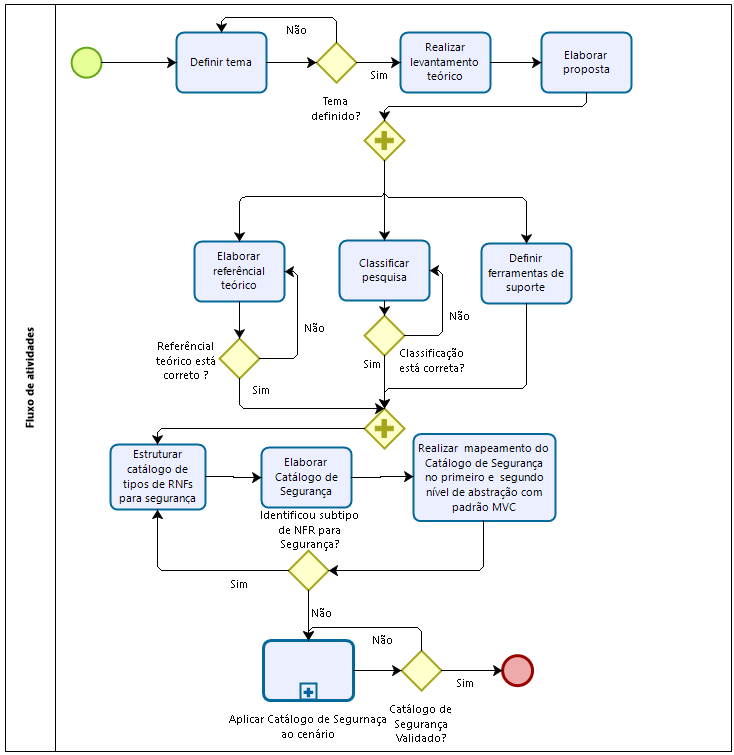
\includegraphics[keepaspectratio=true,scale=0.8]{figuras/fluxodeatividades.PNG}
	\caption{Atividades realizadas.}
	\label{fluxoDeExecuçãoTCC}
\end{figure}

Segue abaixo a descrição das atividades:

\begin{itemize}
	\item \textbf{Definir tema}: em conjunto com os professores orientadores dessa monografia, essa atividade teve como principal objetivo o refinamento sobre os conceitos teóricos referentes à área de interesse do autor;
	
	\item \textbf{Realizar levantamento teórico}: iniciou-se com base nos resultados obtidos na execução da atividade anterior, seguindo as orientações dos orientadores. Discutiu-se sobre os aspectos fundamentais do GORE, os \textit{frameworks} que se apoiam nos conceitos do GORE, os conceitos de Arquitetura de Software e os atributos de qualidade mais relevantes para o mercado e para a academia;
	
	\item \textbf{Elaborar proposta}: com o conhecimento das necessidades da área de atuação desse trabalho, iniciou-se a elaboração da proposta de pequisa, acordando que seria utilizado o NFR \textit{Framework}, bem como, que seria aplicado ao mercado, tomando Segurança como o principal atributo de qualidade;  
	
	\item \textbf{Elaborar referencial teórico}: foi realizada a redação dos conceitos teóricos a serem aplicados no desenvolvimento deste trabalho; 
	
	\item \textbf{Classificar pesquisa}: redação  da classificação da pesquisa em suas dimensões, sendo especificada quanto (i) à abordagem, (ii) à natureza, (iii) aos objetivos, e (iv) aos procedimentos técnicos;
	
	\item \textbf{Definir ferramentas de suporte}: definição e descrição das ferramentas utilizadas no desenvolvimento deste trabalho;
	
	\item \textbf{Estruturar catálogo de tipos de RNFs para Segurança}: com base nos conceitos de Segurança apresentados por Lawrence Chung, Brian A. Nixon, Eric Yu e John Mylopoulos, no  livro: \textit{NON-FUNCTIONAL REQUIREMENTS IN SOFTWARE ENGINEERING}, iniciou-se a elaboração do catálogo de tipos de RNFs para Segurança, expandindo o catálogo com base em definições de subtipos de RNFs;
	
	\item \textbf{Elaborar Catálogo de Segurança}: a partir do Catálogo de Segurança apresentado na Figura \ref{catalogoSegurancaChung}, iniciou-se o processo de identificação das metas flexíveis que podem ser suficientemente satisfeitas, orientando-se também pelo livro supracitado;
	
	\item \textbf{Realizar mapeamento do Catálogo de Segurança no primeiro e segundo nível de abstração com o padrão MVC}: iniciou-se a comparação das metas flexíveis que possuíam relação com o Padrão Arquitetural MVC, a fim de verificar se estas geram impactos, positivos ou negativos, na Segurança dos dados e da arquitetura. Durante a execução dessa atividade, caso ocorresse a identificação de outro subtipo de RNF para Segurança, a atividade “Estruturar catálogo de tipos para Segurança” seria realizada novamente e, consequentemente, as atividades seguintes, de acordo com a Figura \ref{fluxoDeExecuçãoTCC};
	
	\item \textbf{Aplicar Catálogo de Segurança ao cenário}: esta macroatividade respeitou a metodologia de desenvolvimento de software descrito na seção \ref{sec:metodologiaDeDesenvolvimentoDeSoftware}. Haja vista que, em cada ciclo foi definido um cenário com a descrição da persona, identificando, caso necessário, uma possível solução e realizando a aplicação do catálogo. Com isso, realizou-se o desenvolvimento do software, evidenciando a aplicação do catálogo e possibilitando a análise do quanto a Segurança do software pode ser satisfeita, e
	
	\item  \textbf{Realizar mapeamento em terceiro nível de abstração com padrão MVC}: esta atividade foi executada, em paralelo, com o processo de desenvolvimento das aplicações no cenário, onde permitiu aplicar o Catálogo de Segurança e realizar o detalhamento em terceiro nível de abstração, realizando o mapeamento das operacionalizações com as camadas do padrão arquitetural MVC. 
\end{itemize}


\subsection{Cronograma das Atividades}


O cronograma apresentado na Tabela \ref{cronogramaDoTrabalho}, organizado em meses, expõe como se deu a execução das atividades deste trabalho.

\begin{table}[h!]
	\tiny
	\label{cronogramaDoTrabalho}
	\caption{Cronograma de execução do trabalho.}
	\begin{tabular}{@{}lccccccccccccccc@{}}
		\toprule
		\multicolumn{1}{l|}{Ano} & \multicolumn{5}{c|}{\textbf{2017}} & \multicolumn{7}{c|}{\textbf{2018}} & \multicolumn{3}{c}{\textbf{2019}} \\ \midrule
		Atividade/Mês & \textbf{Ago} & \textbf{Set} & \textbf{Out} & \textbf{Nov} & \textbf{Dez} & \textbf{Jan} & \textbf{Fev} & - & \textbf{Ago} & \textbf{Set} & \textbf{Out} & \textbf{Dez} & \textbf{Jan} & \textbf{Fev} & \textbf{Mar} \\ \midrule
		Definir tema & \textbf{x} & \textbf{} & \textbf{} & \textbf{} & \textbf{} & \textbf{} & \textbf{} & - & \textbf{} & \textbf{} & \textbf{} & \textbf{} & \textbf{} & \textbf{} & \textbf{} \\ \midrule
		Elaborar proposta & \textbf{x} & \textbf{x} & \textbf{} & \textbf{} & \textbf{} & \textbf{} & \textbf{} & - & \textbf{} & \textbf{} & \textbf{} & \textbf{} & \textbf{} & \textbf{} & \textbf{} \\ \midrule
		\begin{tabular}[c]{@{}l@{}}Elaborar referencial\\  teórico\end{tabular} & \textbf{x} & \textbf{x} & \textbf{x} & \textbf{x} & \textbf{x} & \textbf{} & \textbf{} & - & \textbf{} & \textbf{} & \textbf{} & \textbf{} & \textbf{} & \textbf{} & \textbf{} \\ \midrule
		Classificar pesquisa & \textbf{} & \textbf{} & \textbf{x} & \textbf{x} & \textbf{x} & \textbf{} & \textbf{} & - & \textbf{} & \textbf{} & \textbf{} & \textbf{} & \textbf{} & \textbf{} & \textbf{} \\ \midrule
		\begin{tabular}[c]{@{}l@{}}Definir ferramentas\\ de suporte\end{tabular} & \textbf{} & \textbf{} & \textbf{x} & \textbf{x} & \textbf{x} & \textbf{} & \textbf{} & - & \textbf{} & \textbf{} & \textbf{} & \textbf{} & \textbf{} & \textbf{} & \textbf{} \\ \midrule
		\begin{tabular}[c]{@{}l@{}}Estruturar Catálogo\\  de Segurança\end{tabular} & \textbf{} & \textbf{} & \textbf{} & \textbf{} & \textbf{x} & \textbf{x} & \textbf{} & - & \textbf{} & \textbf{} & \textbf{} & \textbf{} & \textbf{} & \textbf{} & \textbf{} \\ \midrule
		\begin{tabular}[c]{@{}l@{}}Elaborar Catálogo\\ de Segurança\end{tabular} & \textbf{} & \textbf{} & \textbf{} & \textbf{} & \textbf{x} & \textbf{x} & \textbf{} & - & \textbf{} & \textbf{} & \textbf{} & \textbf{} & \textbf{} & \textbf{} & \textbf{} \\ \midrule
		\begin{tabular}[c]{@{}l@{}}Realizar Mapeamento\\ do Catálogo de\\  Segurança no \\ primeiro e segundo \\ nível de abstração\\ com padrão MVC.\end{tabular} & \textbf{} & \textbf{} & \textbf{} & \textbf{} & \textbf{} & \textbf{x} & \textbf{x} & - & \textbf{} & \textbf{} & \textbf{} & \textbf{} & \textbf{} & \textbf{} & \textbf{} \\ \midrule
		\begin{tabular}[c]{@{}l@{}}Aplicar Catálogo de\\ Segurança ao cenário\end{tabular} & \textbf{} & \textbf{} & \textbf{} & \textbf{} & \textbf{} & \textbf{} & \textbf{} & - & \textbf{x} & \textbf{x} & \textbf{x} & \textbf{x} & \textbf{x} & \textbf{x} & \textbf{} \\ \midrule
		\begin{tabular}[c]{@{}l@{}}Realizar mapeamento \\ em terceiro nível de \\ abstração\end{tabular} & \multicolumn{1}{l}{} & \multicolumn{1}{l}{} & \multicolumn{1}{l}{} & \multicolumn{1}{l}{} & \multicolumn{1}{l}{} & \multicolumn{1}{l}{} & \multicolumn{1}{l}{} & \multicolumn{1}{l}{-} & \textbf{x} & \textbf{x} & \textbf{x} & \textbf{x} & \textbf{x} & \textbf{x} & \textbf{x} \\ \bottomrule
	\end{tabular}
\end{table}

Observa-se que, foram utilizados, além do prazo base para a construção do Catálogo de Segurança, os meses de Janeiro/2018 e Fevereiro/2018. Isso ocorreu para melhor aprofundamento do tema, o qual demandou a leitura de vários materiais bibliográficos. Adicionalmente, as notações envolvidas nessa pesquisa são complexas, o que exige de um cuidado maior na escrita com o objetivo de promover uma melhor compreensão por parte dos interessados.

Com o Catálogo de Segurança concluído, se iniciou o ciclo de aplicação do mesmo em cada cenário. Essa aplicação ocorreu entre o período de Agosto de 2018 a Fevereiro de 2019, haja vista que, alguns cenários eram contextos reais. Dessa forma, somente em março de 2019, foi possível obter o mapeamento no terceiro nível de abstração.

\section{Resumo do Capítulo}

Neste capítulo, foi detalhada na seção \ref{sec:classificacaoDaPesquisa}, a classificação de pesquisa de acordo com seus tipos, sendo estes: (i) abordagem, se tratando de uma pesquisa híbrida, a (ii) Natureza, caraterizada como uma pesquisa aplicada, o (ii) objetivo, caracterizado como uma pesquisa explicativa, e os (iv) procedimentos técnicos, caracterizados como uma pesquisa bibliográfica e a pesquisa-ação. Mais adiante, na seção \ref{sec:metodologiaDeDesenvolvimentoDeSoftware}, foi descrita a adaptação do \textit{Scrum} como metodologia de desenvolvimento de software e o Kanban para acompanhamento visual do andamento do desenvolvimento das aplicações nos cenários. Por fim, na seção \ref{sec:procedimentosMetodológicos}, o fluxo de atividades e o cronograma realizados na execução deste trabalho foram detalhados.

